% academic work by Reza and Alireza Hosseini
% copyright (2015): Reza/Alireza Hosseini
% all this code was generated on authors own time
% authors did not receive any funding
% or were not employed at time of this work
% pdflatex ~/Dropbox/codes/academic/bike_sharing/latex/bike_sharing.tex
\documentclass[11pt,twoside,openany]{article}
\usepackage{
    adjustbox,
	amscd,
	amsbsy,
	amsfonts,
	amsmath,
	amssymb,
	booktabs,
	color,
	enumerate,
    epsfig,
    epstopdf,
	float,
	graphics,
	graphicx,
	geometry,
	latexsym,
	multirow,
	natbib,
    rotating,
    subcaption,
	times,
	verbatim,
	xcolor}


%\usepackage[top=25mm, bottom=25mm, left=37.5mm, right=37.5mm]{geometry}
\graphicspath{
  {figs/}
  {figs/v1/}
  {figs/v2/}
  {diagrams/}
  {emojis/}}

\newcommand{\E}{\mathop{{}\mathbb{E}}}
\newcommand{\var}{\text{Var}}
\newcommand{\bX}{{\bf X}}
\newcommand{\btX}{{\bf \tilde{X}}}
\newcommand{\btY}{{\bf \tilde{Y}}}
\newcommand{\bY}{{\bf Y}}
\newcommand{\bU}{{\bf U}}
\newcommand{\bZ}{{\bf Z}}
\newcommand{\bW}{{\bf W}}
\newcommand{\bWtilde}{{\bf \tilde{W}}}
\newcommand{\btW}{{\bf \tilde{W}}}
\newcommand{\tW}{{\tilde{W}}}
\newcommand{\bbeta}{{\bf \beta}}
\newcommand{\btheta}{{\bf \theta}}
\newcommand{\bPhi}{{\Phi}}
\newcommand{\bepsilon}{{\bf \epsilon}}
\newcommand{\bA}{{\bf A}}
\newcommand{\bphi}{{\bf \phi}}
\newcommand{\btau}{{\bf \tau}}
\newcommand{\bpsi}{{\bf \psi}}
\newcommand{\bPsi}{{\bf \Psi}}
\newcommand{\R}{\mathbb{R}}
\newcommand{\C}{\mathbb{C}}
\newcommand{\F}{\mathbb{F}}
\newcommand{\N}{\mathbb{N}}
\newcommand{\Z}{\mathbb{Z}}
\newcommand{\logit}{\mbox{logit}}
\setlength{\parindent}{12mm}
\setlength{\oddsidemargin}{12mm}
\setlength{\evensidemargin}{12mm}
\setlength{\topmargin}{-7mm}
\setlength{\textwidth}{150mm}
\newcommand{\QED}{\hspace*{\fill}\rule{2.5mm}{2.5mm}}
\newtheorem{theorem}{Theorem}[section]
\newtheorem{definition}{Definition}[section]
\renewcommand{\vec}[1]{\mbox{\boldmath $#1$}}
\newenvironment{proof}{\noindent{\bf Proof\ }}{\QED\\}
\newtheorem{proposition}{Proposition}[section]
\newtheorem{lemma}{Lemma}[section]
\newtheorem{hypothesis}{Hypothesis}[section]
\newtheorem{corollary}{Corollary}[section]
\renewcommand\floatpagefraction{.9}
\renewcommand\topfraction{.9}
\renewcommand\textfraction{.1}
\setcounter{totalnumber}{50}
\setcounter{topnumber}{50}
\setcounter{bottomnumber}{50}
\newcommand{\mysum}{\Sigma}

% to input tables
\newcommand*\inputtable[1]{\input{./tables/#1.tex}}


%\newtheorem{example}{Example}[section]
%\newenvironment{example}[1][Example]{\begin{trivlist}
\begin{document}




\begin{figure}[H]
\centering
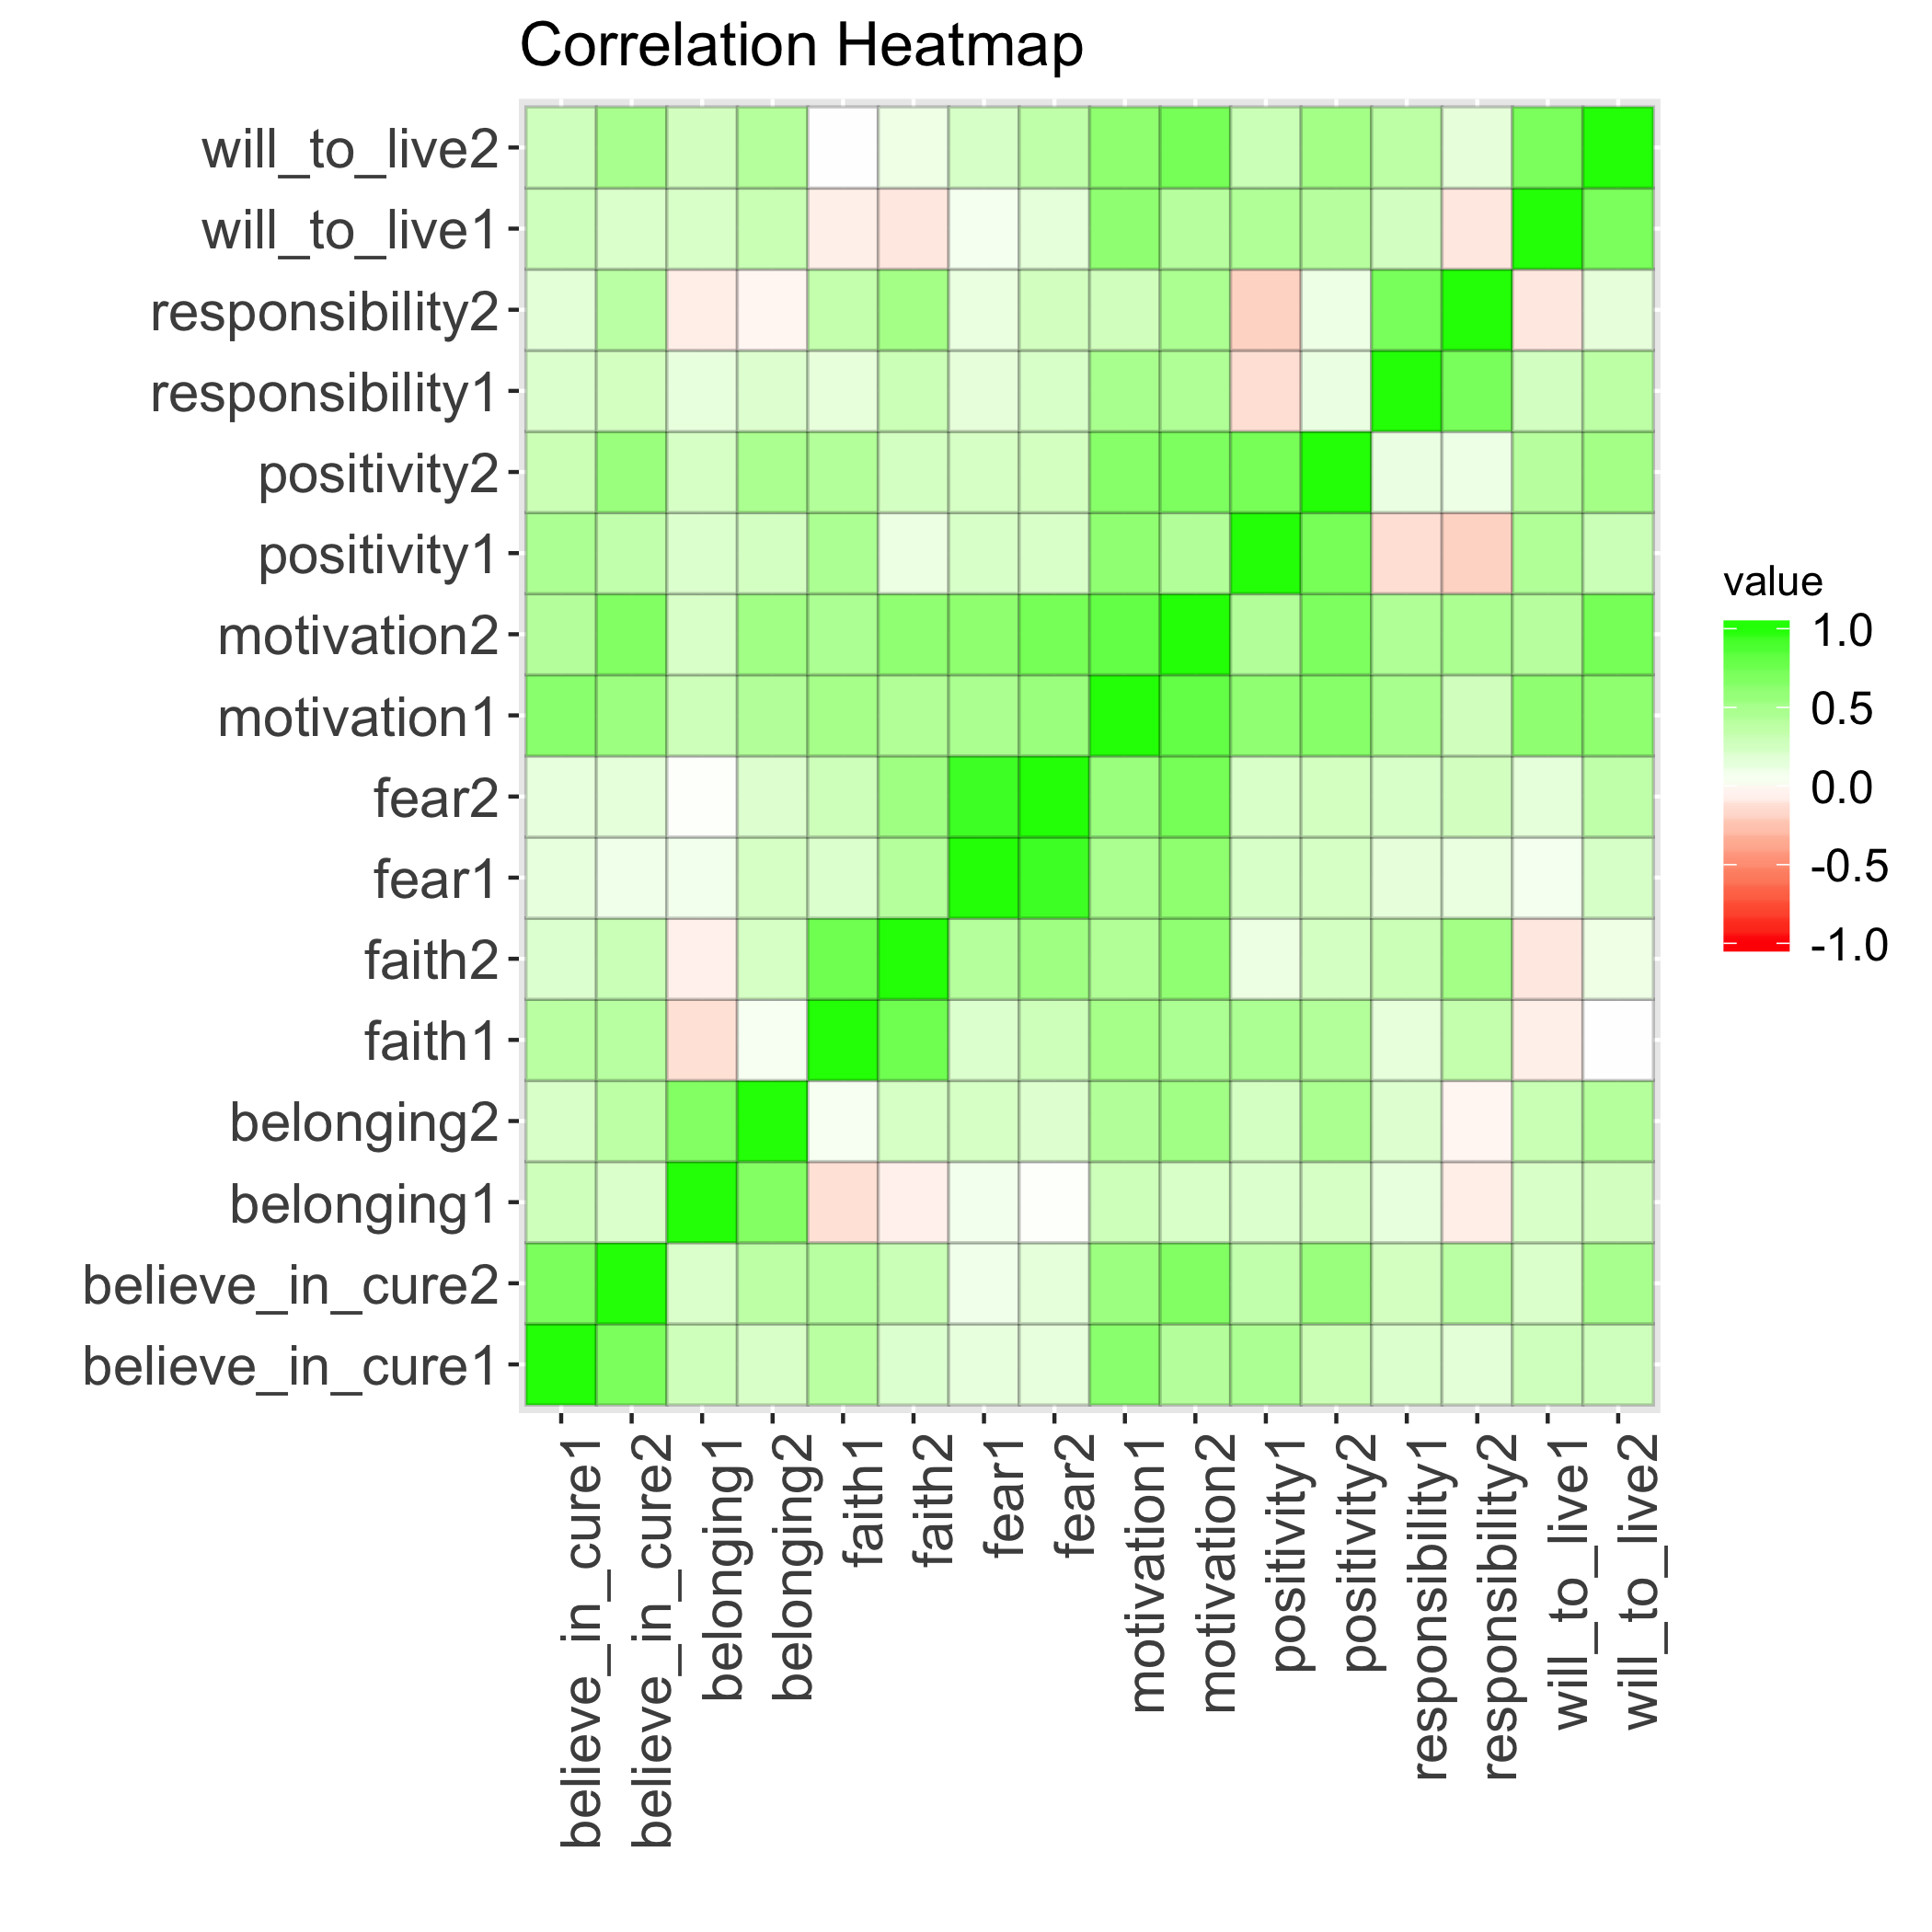
\includegraphics[width=0.5\linewidth]{correlation_over_time.png}
\caption{Correlation over time}
\label{correlation_over_time.png}
\end{figure}


\begin{figure}[H]
\centering
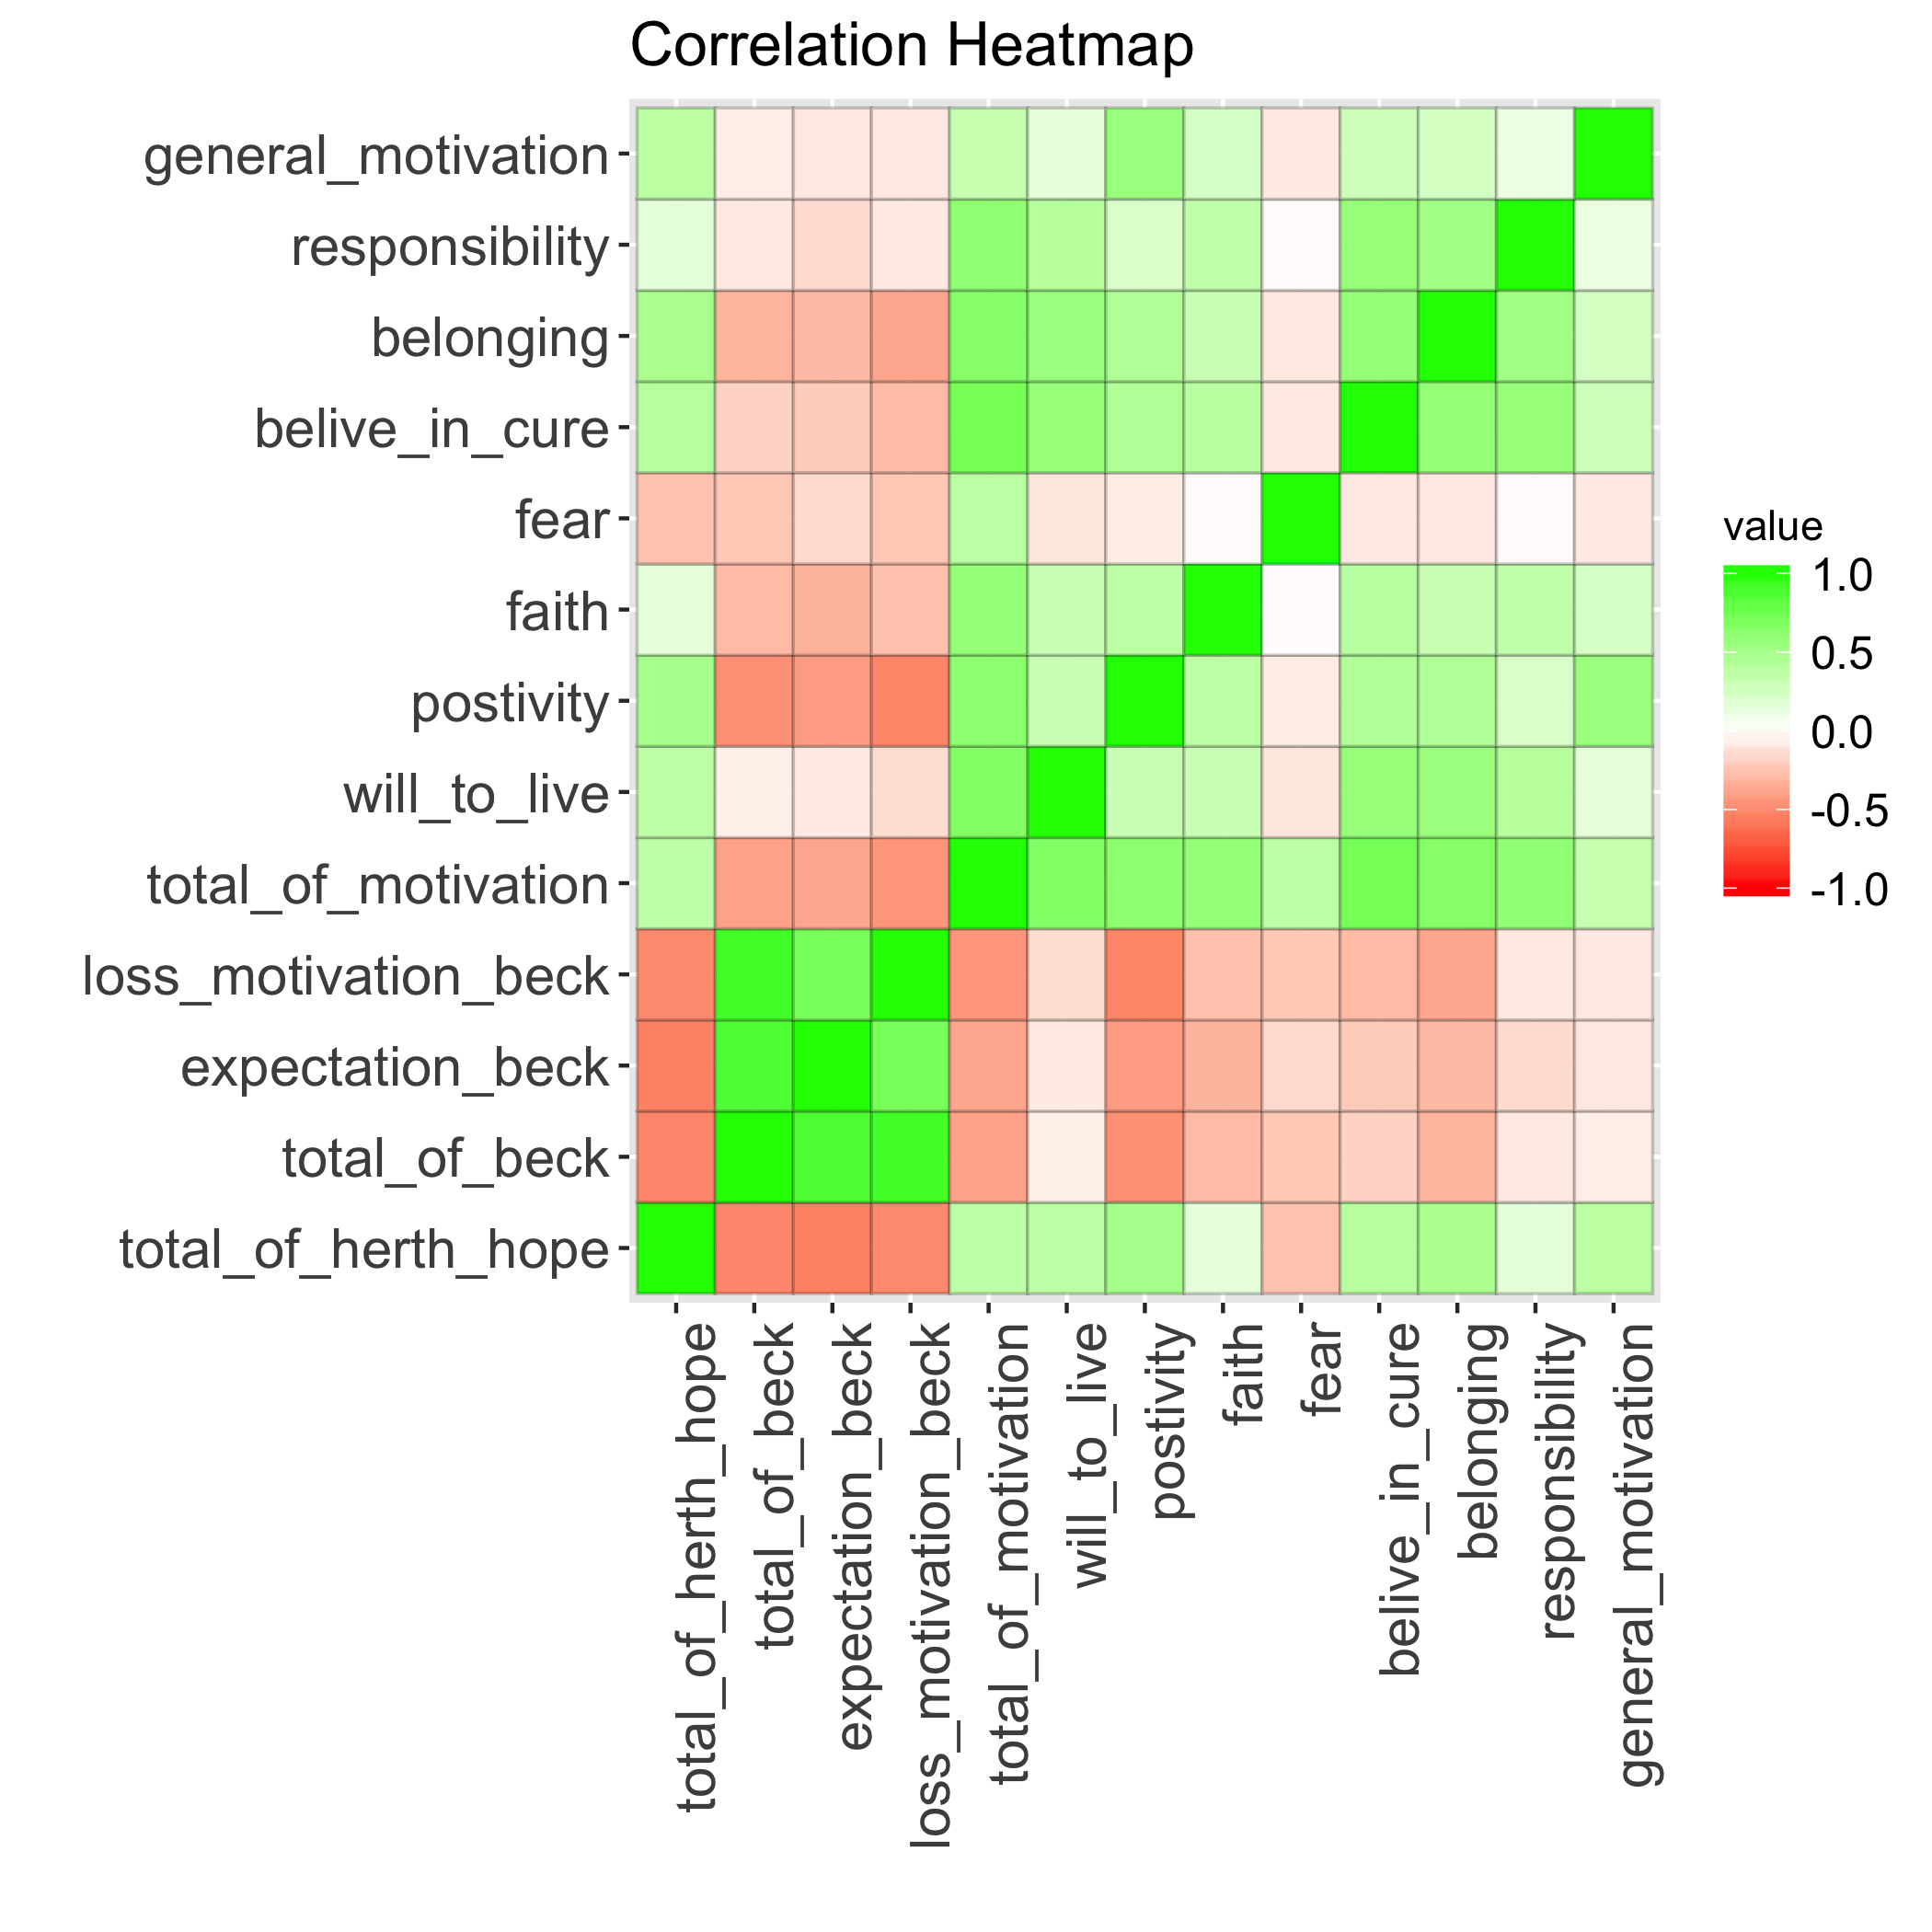
\includegraphics[width=0.5\linewidth]{correlation_across_aggregate_variables.png}
\caption{Correlation across aggregate variables}
\label{correlation_across_aggregate_variables.png}
\end{figure}


% latex table generated in R 3.6.0 by xtable 1.8-4 package
% Thu Dec 24 19:28:48 2020
\begin{table}[ht]
\centering
\begin{tabular}{|r|l|l|}
  \hline
 & Variable & Correlation.CI \\
  \hline
1 & believe\_in\_cure & 42, 86 \\
  2 & belonging & 36, 84 \\
  3 & faith & 51, 89 \\
  4 & fear & 85, 97 \\
  5 & motivation & 60, 91 \\
  6 & positivity & 45, 87 \\
  7 & responsibility & 43, 86 \\ 
  8 & will\_to\_live & 42, 86 \\
   \hline
\end{tabular}
\caption{Correlation over time}
\label{correlation_over_time}
\end{table}


\newpage]

\begin{table}[H] 
\tiny 
 \caption{Correlation conf interval across variables} 
 \label{correlation_conf_interval_across_variables} 
 \centering 
 \begin{adjustbox}{angle=270}  
 \begin{tabular} {|l|l|l|l|l|l|l|l|l|l|l|l|l|l|}  
 \hline 
  &  total\_herth & total\_beck & expect\_beck & motiv\_loss\_beck & total\_motiv & will\_live & positivity & faith & fear & believe\_cure & belonging & responsibility & general\_motiv \\ 
 \hline 
 total\_herth & {\color{green}100,100} & {\color{red}-62,-41} & {\color{red}-64,-44} & {\color{red}-60,-39} & {\color{green}25,49} & {\color{green}25,49} & {\color{green}38,59} & {\color{green}1,28} & {\color{red}-38,-12} & {\color{green}28,52} & {\color{green}36,57} & {\color{green}2,29} & {\color{green}27,50} \\ 
 \hline 
 total\_beck & {\color{red}-62,-41} & {\color{green}100,100} & {\color{green}83,92} & {\color{green}89,95} & {\color{red}-51,-27} & -21,7 & {\color{red}-57,-36} & {\color{red}-41,-16} & {\color{red}-36,-10} & {\color{red}-32,-5} & {\color{red}-43,-19} & -23,5 & -21,6 \\ 
 \hline 
 expect\_beck & {\color{red}-64,-44} & {\color{green}83,92} & {\color{green}100,100} & {\color{green}61,80} & {\color{red}-49,-26} & -23,5 & {\color{red}-53,-30} & {\color{red}-45,-20} & {\color{red}-29,-2} & {\color{red}-35,-9} & {\color{red}-42,-17} & {\color{red}-29,-2} & -23,4 \\ 
 \hline 
 motiv\_loss\_beck & {\color{red}-60,-39} & {\color{green}89,95} & {\color{green}61,80} & {\color{green}100,100} & {\color{red}-56,-34} & -27,0 & {\color{red}-62,-42} & {\color{red}-39,-13} & {\color{red}-36,-10} & {\color{red}-41,-15} & {\color{red}-49,-26} & -23,4 & -23,4 \\ 
 \hline 
 total\_motiv & {\color{green}25,49} & {\color{red}-51,-27} & {\color{red}-49,-26} & {\color{red}-56,-34} & {\color{green}100,100} & {\color{green}57,73} & {\color{green}52,69} & {\color{green}48,66} & {\color{green}25,49} & {\color{green}64,78} & {\color{green}56,72} & {\color{green}50,68} & {\color{green}20,45} \\ 
 \hline 
 will\_live & {\color{green}25,49} & -21,7 & -23,5 & -27,0 & {\color{green}57,73} & {\color{green}100,100} & {\color{green}18,43} & {\color{green}17,42} & -24,3 & {\color{green}47,65} & {\color{green}46,65} & {\color{green}29,52} & {\color{green}2,29} \\ 
 \hline 
 positivity & {\color{green}38,59} & {\color{red}-57,-36} & {\color{red}-53,-30} & {\color{red}-62,-42} & {\color{green}52,69} & {\color{green}18,43} & {\color{green}100,100} & {\color{green}25,49} & -21,6 & {\color{green}32,55} & {\color{green}32,54} & {\color{green}9,35} & {\color{green}45,65} \\ 
 \hline 
 faith & {\color{green}1,28} & {\color{red}-41,-16} & {\color{red}-45,-20} & {\color{red}-39,-13} & {\color{green}48,66} & {\color{green}17,42} & {\color{green}25,49} & {\color{green}100,100} & -15,12 & {\color{green}27,51} & {\color{green}19,44} & {\color{green}23,47} & {\color{green}10,36} \\ 
 \hline 
 fear & {\color{red}-38,-12} & {\color{red}-36,-10} & {\color{red}-29,-2} & {\color{red}-36,-10} & {\color{green}25,49} & -24,3 & -21,6 & -15,12 & {\color{green}100,100} & -23,5 & -23,4 & -16,12 & -22,5 \\ 
 \hline 
 believe\_cure & {\color{green}28,52} & {\color{red}-32,-5} & {\color{red}-35,-9} & {\color{red}-41,-15} & {\color{green}64,78} & {\color{green}47,65} & {\color{green}32,55} & {\color{green}27,51} & -23,5 & {\color{green}100,100} & {\color{green}48,66} & {\color{green}46,65} & {\color{green}16,41} \\ 
 \hline 
 belonging & {\color{green}36,57} & {\color{red}-43,-19} & {\color{red}-42,-17} & {\color{red}-49,-26} & {\color{green}56,72} & {\color{green}46,65} & {\color{green}32,54} & {\color{green}19,44} & -23,4 & {\color{green}48,66} & {\color{green}100,100} & {\color{green}42,62} & {\color{green}11,37} \\ 
 \hline 
 responsibility & {\color{green}2,29} & -23,5 & {\color{red}-29,-2} & -23,4 & {\color{green}50,68} & {\color{green}29,52} & {\color{green}9,35} & {\color{green}23,47} & -16,12 & {\color{green}46,65} & {\color{green}42,62} & {\color{green}100,100} & -2,25 \\ 
 \hline 
 general\_motiv & {\color{green}27,50} & -21,6 & -23,4 & -23,4 & {\color{green}20,45} & {\color{green}2,29} & {\color{green}45,65} & {\color{green}10,36} & -22,5 & {\color{green}16,41} & {\color{green}11,37} & -2,25 & {\color{green}100,100} \\ 
 \hline 
 \hline 
 \end{tabular} 
\end{adjustbox}  
\end{table} 

\begin{table}[H] 
\tiny 
 \caption{Correlation conf interval across variables} 
 \label{correlation_conf_interval_across_variables} 
 \centering 
 \begin{adjustbox}{angle=270}  
 \begin{tabular} {|l|l|l|l|l|l|l|l|l|l|l|l|l|l|}  
 \hline 
  &  total\_herth & total\_beck & expect\_beck & motiv\_loss\_beck & total\_motiv & will\_live & positivity & faith & fear & believe\_cure & belonging & responsibility & general\_motiv \\ 
 \hline 
 total\_herth & {\color{green}100,100} & {\color{red}-62,-41} & {\color{red}-64,-44} & {\color{red}-60,-39} & {\color{green}25,49} & {\color{green}25,49} & {\color{green}38,59} & {\color{green}1,28} & {\color{red}-38,-12} & {\color{green}28,52} & {\color{green}36,57} & {\color{green}2,29} & {\color{green}27,50} \\ 
 \hline 
 total\_beck & {\color{red}-62,-41} & {\color{green}100,100} & {\color{green}83,92} & {\color{green}89,95} & {\color{red}-51,-27} & -21,7 & {\color{red}-57,-36} & {\color{red}-41,-16} & {\color{red}-36,-10} & {\color{red}-32,-5} & {\color{red}-43,-19} & -23,5 & -21,6 \\ 
 \hline 
 expect\_beck & {\color{red}-64,-44} & {\color{green}83,92} & {\color{green}100,100} & {\color{green}61,80} & {\color{red}-49,-26} & -23,5 & {\color{red}-53,-30} & {\color{red}-45,-20} & {\color{red}-29,-2} & {\color{red}-35,-9} & {\color{red}-42,-17} & {\color{red}-29,-2} & -23,4 \\ 
 \hline 
 motiv\_loss\_beck & {\color{red}-60,-39} & {\color{green}89,95} & {\color{green}61,80} & {\color{green}100,100} & {\color{red}-56,-34} & -27,0 & {\color{red}-62,-42} & {\color{red}-39,-13} & {\color{red}-36,-10} & {\color{red}-41,-15} & {\color{red}-49,-26} & -23,4 & -23,4 \\ 
 \hline 
 total\_motiv & {\color{green}25,49} & {\color{red}-51,-27} & {\color{red}-49,-26} & {\color{red}-56,-34} & {\color{green}100,100} & {\color{green}57,73} & {\color{green}52,69} & {\color{green}48,66} & {\color{green}25,49} & {\color{green}64,78} & {\color{green}56,72} & {\color{green}50,68} & {\color{green}20,45} \\ 
 \hline 
 will\_live & {\color{green}25,49} & -21,7 & -23,5 & -27,0 & {\color{green}57,73} & {\color{green}100,100} & {\color{green}18,43} & {\color{green}17,42} & -24,3 & {\color{green}47,65} & {\color{green}46,65} & {\color{green}29,52} & {\color{green}2,29} \\ 
 \hline 
 positivity & {\color{green}38,59} & {\color{red}-57,-36} & {\color{red}-53,-30} & {\color{red}-62,-42} & {\color{green}52,69} & {\color{green}18,43} & {\color{green}100,100} & {\color{green}25,49} & -21,6 & {\color{green}32,55} & {\color{green}32,54} & {\color{green}9,35} & {\color{green}45,65} \\ 
 \hline 
 faith & {\color{green}1,28} & {\color{red}-41,-16} & {\color{red}-45,-20} & {\color{red}-39,-13} & {\color{green}48,66} & {\color{green}17,42} & {\color{green}25,49} & {\color{green}100,100} & -15,12 & {\color{green}27,51} & {\color{green}19,44} & {\color{green}23,47} & {\color{green}10,36} \\ 
 \hline 
 fear & {\color{red}-38,-12} & {\color{red}-36,-10} & {\color{red}-29,-2} & {\color{red}-36,-10} & {\color{green}25,49} & -24,3 & -21,6 & -15,12 & {\color{green}100,100} & -23,5 & -23,4 & -16,12 & -22,5 \\ 
 \hline 
 believe\_cure & {\color{green}28,52} & {\color{red}-32,-5} & {\color{red}-35,-9} & {\color{red}-41,-15} & {\color{green}64,78} & {\color{green}47,65} & {\color{green}32,55} & {\color{green}27,51} & -23,5 & {\color{green}100,100} & {\color{green}48,66} & {\color{green}46,65} & {\color{green}16,41} \\ 
 \hline 
 belonging & {\color{green}36,57} & {\color{red}-43,-19} & {\color{red}-42,-17} & {\color{red}-49,-26} & {\color{green}56,72} & {\color{green}46,65} & {\color{green}32,54} & {\color{green}19,44} & -23,4 & {\color{green}48,66} & {\color{green}100,100} & {\color{green}42,62} & {\color{green}11,37} \\ 
 \hline 
 responsibility & {\color{green}2,29} & -23,5 & {\color{red}-29,-2} & -23,4 & {\color{green}50,68} & {\color{green}29,52} & {\color{green}9,35} & {\color{green}23,47} & -16,12 & {\color{green}46,65} & {\color{green}42,62} & {\color{green}100,100} & -2,25 \\ 
 \hline 
 general\_motiv & {\color{green}27,50} & -21,6 & -23,4 & -23,4 & {\color{green}20,45} & {\color{green}2,29} & {\color{green}45,65} & {\color{green}10,36} & -22,5 & {\color{green}16,41} & {\color{green}11,37} & -2,25 & {\color{green}100,100} \\ 
 \hline 
 \hline 
 \end{tabular} 
\end{adjustbox}  
\end{table} 
 
\begin{table}[H] 
\tiny 
 \caption{Correlation conf interval across variables} 
 \label{correlation_conf_interval_across_variables} 
 \centering 
 \begin{adjustbox}{angle=270}  
 \begin{tabular} {|l|l|l|l|l|l|l|l|l|l|l|l|l|l|}  
 \hline 
  &  total\_herth & total\_beck & expect\_beck & motiv\_loss\_beck & total\_motiv & will\_live & positivity & faith & fear & believe\_cure & belonging & responsibility & general\_motiv \\ 
 \hline 
 total\_herth & {\color{green}100,100} & {\color{red}-62,-41} & {\color{red}-64,-44} & {\color{red}-60,-39} & {\color{green}25,49} & {\color{green}25,49} & {\color{green}38,59} & {\color{green}1,28} & {\color{red}-38,-12} & {\color{green}28,52} & {\color{green}36,57} & {\color{green}2,29} & {\color{green}27,50} \\ 
 \hline 
 total\_beck & {\color{red}-62,-41} & {\color{green}100,100} & {\color{green}83,92} & {\color{green}89,95} & {\color{red}-51,-27} & -21,7 & {\color{red}-57,-36} & {\color{red}-41,-16} & {\color{red}-36,-10} & {\color{red}-32,-5} & {\color{red}-43,-19} & -23,5 & -21,6 \\ 
 \hline 
 expect\_beck & {\color{red}-64,-44} & {\color{green}83,92} & {\color{green}100,100} & {\color{green}61,80} & {\color{red}-49,-26} & -23,5 & {\color{red}-53,-30} & {\color{red}-45,-20} & {\color{red}-29,-2} & {\color{red}-35,-9} & {\color{red}-42,-17} & {\color{red}-29,-2} & -23,4 \\ 
 \hline 
 motiv\_loss\_beck & {\color{red}-60,-39} & {\color{green}89,95} & {\color{green}61,80} & {\color{green}100,100} & {\color{red}-56,-34} & -27,0 & {\color{red}-62,-42} & {\color{red}-39,-13} & {\color{red}-36,-10} & {\color{red}-41,-15} & {\color{red}-49,-26} & -23,4 & -23,4 \\ 
 \hline 
 total\_motiv & {\color{green}25,49} & {\color{red}-51,-27} & {\color{red}-49,-26} & {\color{red}-56,-34} & {\color{green}100,100} & {\color{green}57,73} & {\color{green}52,69} & {\color{green}48,66} & {\color{green}25,49} & {\color{green}64,78} & {\color{green}56,72} & {\color{green}50,68} & {\color{green}20,45} \\ 
 \hline 
 will\_live & {\color{green}25,49} & -21,7 & -23,5 & -27,0 & {\color{green}57,73} & {\color{green}100,100} & {\color{green}18,43} & {\color{green}17,42} & -24,3 & {\color{green}47,65} & {\color{green}46,65} & {\color{green}29,52} & {\color{green}2,29} \\ 
 \hline 
 positivity & {\color{green}38,59} & {\color{red}-57,-36} & {\color{red}-53,-30} & {\color{red}-62,-42} & {\color{green}52,69} & {\color{green}18,43} & {\color{green}100,100} & {\color{green}25,49} & -21,6 & {\color{green}32,55} & {\color{green}32,54} & {\color{green}9,35} & {\color{green}45,65} \\ 
 \hline 
 faith & {\color{green}1,28} & {\color{red}-41,-16} & {\color{red}-45,-20} & {\color{red}-39,-13} & {\color{green}48,66} & {\color{green}17,42} & {\color{green}25,49} & {\color{green}100,100} & -15,12 & {\color{green}27,51} & {\color{green}19,44} & {\color{green}23,47} & {\color{green}10,36} \\ 
 \hline 
 fear & {\color{red}-38,-12} & {\color{red}-36,-10} & {\color{red}-29,-2} & {\color{red}-36,-10} & {\color{green}25,49} & -24,3 & -21,6 & -15,12 & {\color{green}100,100} & -23,5 & -23,4 & -16,12 & -22,5 \\ 
 \hline 
 believe\_cure & {\color{green}28,52} & {\color{red}-32,-5} & {\color{red}-35,-9} & {\color{red}-41,-15} & {\color{green}64,78} & {\color{green}47,65} & {\color{green}32,55} & {\color{green}27,51} & -23,5 & {\color{green}100,100} & {\color{green}48,66} & {\color{green}46,65} & {\color{green}16,41} \\ 
 \hline 
 belonging & {\color{green}36,57} & {\color{red}-43,-19} & {\color{red}-42,-17} & {\color{red}-49,-26} & {\color{green}56,72} & {\color{green}46,65} & {\color{green}32,54} & {\color{green}19,44} & -23,4 & {\color{green}48,66} & {\color{green}100,100} & {\color{green}42,62} & {\color{green}11,37} \\ 
 \hline 
 responsibility & {\color{green}2,29} & -23,5 & {\color{red}-29,-2} & -23,4 & {\color{green}50,68} & {\color{green}29,52} & {\color{green}9,35} & {\color{green}23,47} & -16,12 & {\color{green}46,65} & {\color{green}42,62} & {\color{green}100,100} & -2,25 \\ 
 \hline 
 general\_motiv & {\color{green}27,50} & -21,6 & -23,4 & -23,4 & {\color{green}20,45} & {\color{green}2,29} & {\color{green}45,65} & {\color{green}10,36} & -22,5 & {\color{green}16,41} & {\color{green}11,37} & -2,25 & {\color{green}100,100} \\ 
 \hline 
 \hline 
 \end{tabular} 
\end{adjustbox}  
\end{table} 
 




\end{document}
